\chapter{The Value of Information}\label{chap:chengdu}
\epigraph{Compared to dispatching where the vehicle transitions are determined by the origins and destinations of the outstanding orders, the repositioning operation is a proactive measure that has the freedom to make recommendations of any feasible destinations inside the city. On the flip side, it becomes a much complicated problem when the goal is to improve the average driver income of a large fleet for an extended period of time (e.g., more than 8 hours per day), which often requires some form of coordination among the vehicles to avoid causing undesirable competitions, e.g., crowding too many vehicles into a single high-demand location.}{\cite{Tang2021}}
While the last chapter investigated stated aspects of relevance for labor supply, this section shows the \emph{potential} effects of platform design beyond matching and pricing in the case of information.

We present evidence that demand information can significantly increase earnings for platform drivers. The earnings gains are aligned with claims by companies that offer information services to drivers such as Gridwise or Surge that additional information can increase earnings, compare \cite{Weed2019}. We first describe the data used in our estimation in \autoref{sec:chengdudata}. We then estimate driver earnings in optimized repositioning in \autoref{sec:chengduestimation} and close with comparing this with driver income under non-optimized behavior and discuss our results in \autoref{sec:chengdudiscussion}.
\section{Description of Data}\label{sec:chengdudata}
The DiDi KDD Challenge 2020, sponsored by TNC DiDi, consisted of two challenges. An order dispatch challenge, that asked to match orders to drivers with the goal of maximizing the value of all orders completed, and a driver repositioning challenge that asked to reposition a small number of drivers to maximize the earnings rate of this group of drivers. We will work with data and submissions of the latter challenge.

\subsection{Annotated Order Data}
We use a dataset of 14,131,874 orders dispatched in Chengdu, China, in November 2016. An order consists of an origin-destination pair, a timestamp for beginning and end time, an identifier for the driver that took the order, and a number of \emph{reward units}. Reward units are a proxy for driver income provided by DiDi. As we argue statistically below, reward units are linear transformations of real currency. We recover an approximate translation of reward units into \textyen, the local currency. As of the submission time of this thesis, the data is not available anymore, and the terms do not allow hosting of the data. Hence, we cannot provide replication for this part of our analysis.

\subsection{Evaluation in Paper}
The KDD 2020 reinforcement learning challenge solves an optimal repositioning problem together with an optimal order dispatch problem. We make use of the repositioning scores in the paper \cite{Tang2021}, which solves two dynamic planning problems

For the order dispatch algorithm, the system's observable state consists of a list of orders to be dispatched at each point in time. An order is an origin-destination pair, and for each driver timestamps of \emph{estimated} order pickup and arrival times, as well as the distance for the driver. The available actions are matchings of drivers to orders, which are one-to-one, as the challenge does not consider carpooling. Orders need to be dispatched within two seconds, otherwise they are lost. (We specify the complete state in in \autoref{app:kdd}. As part of the state transitions, there is estimated data for cancellation probabilities when sending a driver to pick up orders from different locations.

The objective in the order dispatch challenge is to maximize average driver income.

The system's observable state for the driver repositioning challenge, which we are using in this chapter, consists of a set of drivers to be repositioned. A driver becomes eligible for repositioning after five minutes of being idle if they are in a small group of \emph{treated drivers}. In addition to a timestamp, the only information given on drivers is a coarse position on a hexagonal grid of the urban area of Chengdu. The actions are matchings of drivers to destination locations. Drivers move to their destination at 3m/s in the spherical/great arc distance. Idle drivers move according to historical transition probabilities between regions before being idle for 5 minutes or non-targeted.

The objective in the driver repositioning problem is to maximize mean driver income rate for drivers. Denote $L_k^n (\pi)$ the online time for driver $k$ at day $n$ in hours.\footnote{While the existing documentation do not specify the unit of this measure, our calculations below show that assuming online time is measured in hours leads to correct results.} Denote driver $k$'d income on day $n$ under policy $\pi$ by $J_k^n (\pi)$. For the set of all targeted drivers $K$ and days $N$, the goal of the challenge is to maximize the earnings rate of repositioned drivers,
\begin{equation}
	\frac{1}{\lvert K\rvert} \sum_{k \in K} \frac{\sum_{n \in N} J_k^n (\pi)}{\sum_{n \in N} L_k^n (\pi)}.\label{eq:repositioningscore}
\end{equation}
The optimal repositioning score for drivers is informative for the value of demand information for drivers. If drivers have sufficient information about the demand throughout the city, they can reposition themselves to another location in expectation of getting higher earnings. In contrast to the platform's incentive of maximizing the volume of orders completed, the repositioning challenges maximizes driver earnings taking into account periods 1, 2, and 3, and hence reflects the earnings rate that a perfectly informed driver would receive.

In this argument, the smallness number of repositioned drivers is important. A challenge for drivers, but not for the platform, is that a knowledge on high demand in some area might lead to congestive effects---too many drivers enter high-demand areas. We will discuss this point more thoroughly in \autoref{chap:infodesign}.

\cite{Tang2021} finds, compare their Fig. 3(a), that a policy that samples transition probabilities for a time of day from historical data reaches a repositioning score of about 8.5, whereas the earnings from their best tested repositioning policy gave a score of 9.

\subsection{Earnings Table}
We use a publicly available table for earnings from 2021 \cite{Icauto.com2021}. In 2017, DiDi introduced two tiers of service for their drivers, Economic Express and Economic Premium. After personal conversations with experts in the market, we will use the earnings for the Economic Express tier as proxy for November 2016 earnings. We reproduce the table in \autoref{tab:earnings}. 

The earnings table contains, dependent of the time of the day, a base price $b_t$, earnings per kilometer $l_t$ from the third cilometer and minute driven $d_t$ from the fifth minute. At the time of the data, November 2016, additionally, a surge multiplier $s_t$ which is not part of the table. The total earnings $e_t$ for a ride of $L$ kilometers and duration $D$ are given by 
\begin{equation}
	e_t = s_t(b_t + l_t L + d_t D).\label{eq:earnings}
\end{equation}
\begin{table}[]
\centering
\begin{tabular}{lllll}
\toprule
 & Base Price & Price/km & Price/min &  \\
\midrule
$22:00-07:00$  & 12.40      & 2.70     & 0.48      &  \\
$07:00-10:00$  & 12.40      & 2.55     & 0.48      &  \\
$10:00-16:00$ & 11.40      & 1.95     & 0.42      &  \\
$16:00-19:00$ & 12.40      & 2.33     & 0.48      &  \\
$19:00-22:00$ & 11.40      & 1.95     & 0.42      & \\
\bottomrule
\end{tabular}
\caption{Earnings for DiDi Economic Express drivers.}\label{tab:earningstable}
\end{table}
\section{Estimation}\label{sec:chengduestimation}
We will estimate a linear relationship of earnings and reward units, and test the linearity of the relationship. 
\subsection{Estimation}\label{subsec:chengduregress}
We estimate the equation \eqref{eq:earnings},
\[
	e_t = b_t + l_t L + d_t D.
\]
for $t$ dependent on the different time periods in \autoref{tab:earningstable}, 
\[
t \in \{\text{22:00-07:00},\text{07:00-10:00},\text{10:00-16:00},\text{16:00-19:00},\text{19:00-22:00}\}
\]
as well as a simpler model 
\[
	e = b + l L + d D
\]
which disregards these periods. We use the Google Maps API to estimate driving distance associated with trips and the DiDi provided duration as duration. The estimation results are presented in \autoref{tab:rewardunits}. We find highly significant and consistent estimates on the coefficients for distance and duration and a very strong effect ($R^2 = 0.887$). The Harvey-Collier test for linearity of a model \cite{Harvey1977}, we are unable to reject the Null Hypothesis of linearity ($p = 0.56$). This means, that our assumption of a linear relationship between reward units and earnings cannot be rejected in the data.
\begin{table}[!htbp] \centering
\begin{tabular}{@{\extracolsep{5pt}}lcc}
\\[-1.8ex]\hline
\hline \\[-1.8ex]
& \multicolumn{2}{c}{Dependent variable: Reward Units} \
\cr \cline{2-3}
\\[-1.8ex] & (1) & (2) \\
\hline \\[-1.8ex]
 Intercept & 0.751$^{***}$ & 0.703$^{***}$ \\
  & (0.042) & (0.041) \\
 distance & 0.290$^{***}$ & 0.317$^{***}$ \\
  & (0.014) & (0.076) \\
 duration & 0.065$^{***}$ & 0.116$^{***}$ \\
  & (0.005) & (0.041) \\
 hour[T.22-7]:distance & & -0.043$^{}$ \\
  & & (0.077) \\
 hour[T.22-7]:duration & & -0.050$^{}$ \\
  & & (0.041) \\
 hour[T.7-10]:distance & & -0.067$^{}$ \\
  & & (0.089) \\
 hour[T.7-10]:duration & & -0.037$^{}$ \\
  & & (0.043) \\
 hour[T.offhour]:distance & & 0.003$^{}$ \\
  & & (0.078) \\
 hour[T.offhour]:duration & & -0.057$^{}$ \\
  & & (0.041) \\
\hline \\[-1.8ex]
 Observations & 3,997 & 3,997 \\
 $R^2$ & 0.883 & 0.894 \\
 Adjusted $R^2$ & 0.883 & 0.894 \\
\hline
\hline \\[-1.8ex]
\textit{Note:} & \multicolumn{2}{r}{$^{*}$p$<$0.1; $^{**}$p$<$0.05; $^{***}$p$<$0.01} \\
\end{tabular}
\caption{Reward unit regression}\label{tab:rewardunits}
\end{table}
The $F$-statistic of the smaller is much larger than the one of the larger model ($2911.7$ vs. $1074.8$), which means that all differences in hour-dependent pay are non-significant. As we do not have access to data from Changdu, we cannot determine whether this is a result of surge prices cancelling earnings variations or caused by the absence of price variations between hours. We will proceed by using the smaller model. 

This allows us to estimate driver earnings for orders. By comparing the base price, per-kilometer and per-minute prices with our earnings, we get three estimates of \textyen/reward unit: 11.4/0.751 = 15.2, 1.95/0.29 = 6.7, and 0.42/0.0065 = 6.5. We will, in our estimations, use the average of the latter two, 6.6, assuming that the base price for drivers in Chengdu has decreased since 2017. Note that this is a very conservative estimate given that the rate would be much higher when calibrating against the base rate.

We assume that the earnings rate as given in \eqref{eq:repositioningscore} are estimated per hour. Given the data available, we are not able to calibrate whether this is correct.

Using our estimation, we can estimate the performance of the human expert policy as $8.5 \text{reward units}/\text{hour} \cdot 6.6 \frac{\text{\textyen}}{\text{reward units}} = 56.1 \text{\textyen}$. This lies in the band of first and second tier Chinese cities, for which average hourly income of 40-60 \textyen are reported \cite{DayDayNews2019a}. The optimal repositioning gives earnings of $9 \text{reward units}/\text{hour} \cdot 6.6 \frac{\text{\textyen}}{\text{reward units}} = 59.4 \text{\textyen}$ which is on the upper end of the interval, which means a significant earnings increase of 3.3 \textyen per hour.

As another check of our model fit and immediate use of our model, we infer the distribution of surge prices throughout the day. We use the estimated values \autoref{tab:rewardunits} to calculate a quantity of raw earnings $r_t = \overline{l}L + \overline{d}D =  0.290 L + 0.065D$. We then regress earnings
\[
e_t = \beta_t r_t
\]
and find the surge multipliers given in \autoref{fig:surge}, which emphasize the evening rush hour, but do not show as pronounced of a morning rush hour. 
\begin{figure}
\centering
% This file was created by tikzplotlib v0.9.9.
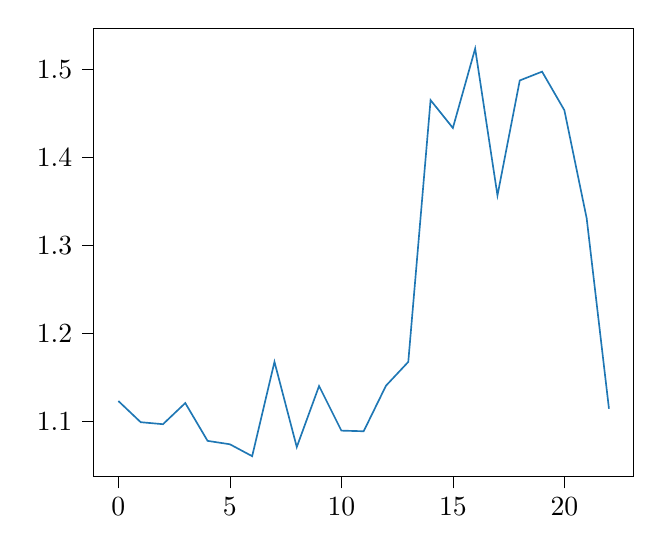
\begin{tikzpicture}

\definecolor{color0}{rgb}{0.12156862745098,0.466666666666667,0.705882352941177}

\begin{axis}[
tick align=outside,
tick pos=left,
x grid style={white!69.0196078431373!black},
xmin=-1.1, xmax=23.1,
xtick style={color=black},
y grid style={white!69.0196078431373!black},
ymin=1.03735226255502, ymax=1.5468767393805,
ytick style={color=black}
]
\addplot [semithick, color0]
table {%
0 1.12318495198341
1 1.09913427730735
2 1.09685008933075
3 1.12089978526511
4 1.07791360444631
5 1.07404308128588
6 1.06051246604709
7 1.16772775842556
8 1.07086755547742
9 1.14025887467618
10 1.08954673715514
11 1.08882563810095
12 1.14058285016778
13 1.16764119140973
14 1.46517891466457
15 1.43351301329444
16 1.52371653588844
17 1.35688942240336
18 1.48752586983921
19 1.49753065470143
20 1.45369418882321
21 1.33089520382377
22 1.11446109300405
};
\end{axis}

\end{tikzpicture}

\caption{Estimate average surge multipliers throughout the day.}\label{fig:surge}	
\end{figure}

\section{Discussion}\label{sec:chengdudiscussion}
We find that optimal driver repositioning has a significant, but not too large effect on driver earnings if only a few drivers are treated to this additional information. 

In a model with more drivers being treated, informed drivers might \emph{crowd out} each other, and earnings differential might be smaller.

This does not mean that information design is not possible to improve platforms, but that, for each trip, only a subset of drivers may be informed of it. This robust property is one of our findings in the next chapter.